
\ifintegriereaufgaben

\section*{Systemanalyse Aufgaben}\label{MA2-systemanalyse-aufgaben}
Regeln und Beispiele, die zur Bearbeitung der Aufgaben hilfreich sind, finden Sie im Skript\wennreferenzvorhanden{MA2-systemanalyse}{ (Abschnitt \abschnittsverweis{MA2-systemanalyse})} und, falls Sie nicht weiterkommen, schauen Sie \hyperref[MA2-systemanalyse-loesungen]{hier}.
\else
\section{Systemanalyse Aufgaben}\label{MA2-systemanalyse-aufgaben}

Regeln und Beispiele zu diesen Aufgaben finden Sie im Skript. Die L�sungen finden Sie \hyperref[MA2-systemanalyse-loesungen]{hier}.
\fi

\begin{exercisebox}[Polstellen (�bertragungsfunktion Laplace) ] % s=-1, s=-2
Gegeben sei

\[
H(s)=\frac{2}{s^2+3s+2}.
\]

\begin{enumerate}

\item Bestimmen Sie die Polstellen von \(H(s)\).

\item Skizzieren Sie die Lage der Polstellen in der komplexen Ebene.

\end{enumerate}


\end{exercisebox}

\begin{exercisebox}[Polstellen (�bertragungsfunktion Laplace)] % s = -1 pm 2i
Gegeben sei

\[
H(s)=\frac{1}{s^2+2s+5}.
\]

\begin{enumerate}

\item Bestimmen Sie die Polstellen.

\item Skizzieren Sie die Lage der Polstellen in der komplexen Ebene.

\item Was bedeutet das f�r das Zeitverhalten eines Systems?

\end{enumerate}

\end{exercisebox}

\begin{exercisebox}[Polstellen (�bertragungsfunktion Laplace)] % s = -1 pm 2i
Die folgende Skizze zeigt die Polstellen einer �bertragungsfunktion in der komplexen Ebene.

\begin{center}
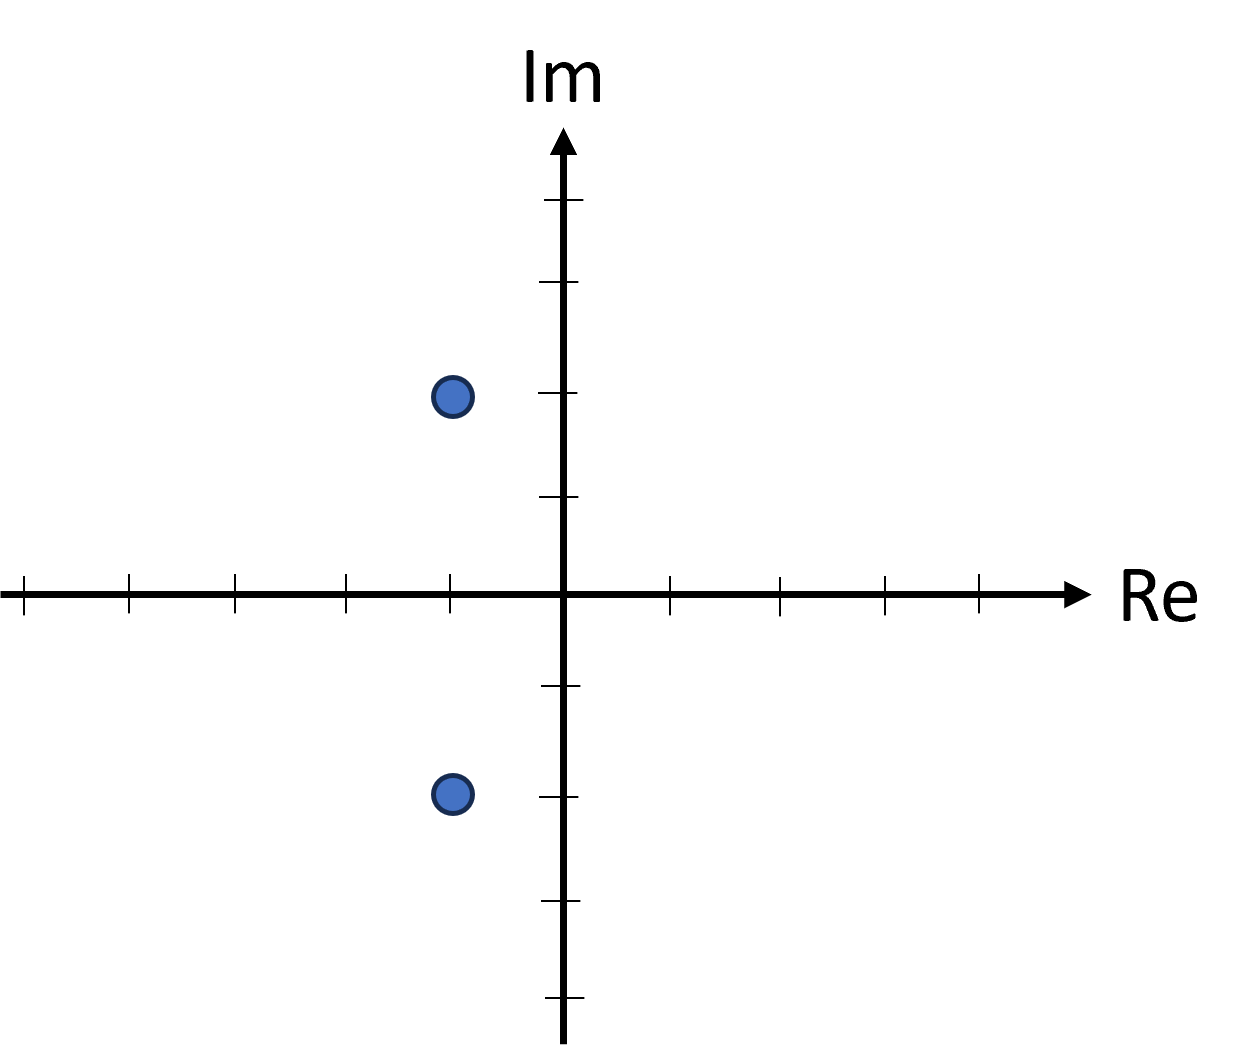
\includegraphics[width=5cm]{../Mathematik_2/Bilder/systemanalyse_konjugiert_komplexe_polstellen.png}
\end{center}

\begin{enumerate}
\item Lesen Sie die Polstellen aus der Skizze ab.
\item Geben Sie ein m�gliches Polynom an, das im Nenner der �bertragungsfunktion stehen k�nnte.
\end{enumerate}

\end{exercisebox}

